\section{Ranking Classes and Safety}
\label{sec:nexthop}

In this section, we study two natural ranking classes under which ASes
retain autonomy in setting rankings over paths.  First, in Section
\ref{ssec:nhp}, we study the
rankings where each AS is allowed to rank paths solely
based on the immediate next-hop AS, called ``next-hop rankings''.  We show that (1)~there are routing systems where
each node has only a next-hop ranking that are not safe;
and (2)~even though all routing systems where nodes have next-hop
rankings are stable, there exist some routing systems of
this form that are not stable under filtering.  

In Section
\ref{ssec:ew}, we study the
properties of routing systems where each node is allowed to choose a
weight for all its outgoing links, and rankings are
derived from a ``total'' weight associated to each path.  The total weight of a
path is defined as the weight of the first link on that path, plus a
discounted sum of the weights of all remaining links on that path.  We
show that if the discount factor is anything other than $1$ (which
corresponds to shortest path routing), then there exist weight configurations
that yield a routing system that is not safe.

\subsection{Next-Hop Rankings}
\label{ssec:nhp}

One natural set of rankings for a routing system is one where each AS
can express rankings over paths solely based on the next-hop AS in
the path.  
Such a class of rankings makes sense because an AS establishes
bilateral contracts with its immediate neighbors and, as such, will most
often wish
to configure its rankings based on the immediate next-hop AS en route
to the destination.  For example, an AS will typically prefer sending
traffic via routes through its neighboring customer ASes over other
ASes, since those customer ASes are paying based on traffic volume. 
We formally define next-hop rankings as follows:

\begin{defn}[Next-hop ranking]
\label{def:next-hop}
Given $N$, $\prec_i$ is a {\em next-hop ranking} if, for all nodes $j,
k$ with $i,j,k$ distinct, we have: 
\begin{equation}
\label{eq:nh}
i j P_j 0 \prec_i i k P_k 0\ \Rightarrow  i j P'_j 0 \prec_i i k P'_k
0,
\end{equation}
for all $P_j, P'_j \in \P_j^N$, and $P_k, P'_k \in \P_k^N$.
(Here we interpret $\P_0^N = \{ \epsilon \}$.)
%
Thus, $\prec_i$ ranks paths based only on the first hop of each path.
\end{defn}

Such a restriction on policy would still be sufficiently rich to achieve
most traffic engineering goals, since most policies are based on the
immediate next-hop AS~\cite{Feamster2003e}.  Additionally, this class of
rankings is expressive enough for most current policy goals,
because most current routing policies are dictated according to the AS's
business relationship with its immediate neighbor.  In this section,
we show that while systems with next-hop rankings are generally
stable, there exist examples that are unsafe, as well as systems that
are unstable under filtering.

In the following proposition, we routing systems with next-hop rankings,
provided that no filtering is employed.  The proof is straightforward,
using a construction due to Feigenbaum \ea\cite{Feigenbaum2004}.
%Details can be found in \cite{Feamster05}.

\begin{prop}
Suppose $(N, \prec_1, \ldots, \prec_N, \F_1, \ldots, \F_N)$ is a
routing system such that $\prec_i$ is a next-hop ranking for each $i$,
and $\F_i = \P_i$ for all $i$.  Then there exists a stable path
assignment $\v{P}$ for this routing system.
\end{prop}

We now show that there may exist 
$\hat{\F}_1 \ldots \hat{\F}_N$, where $\hat{\F}_i \subseteq \F_i$
for all $i$, such that even though the system $(N, \prec_1 \ldots
\prec_N, \F_1 \ldots \F_N)$ is stable, the filtered system $(N,
\prec_1 \ldots \prec_N, \hat{\F}_1 \ldots \hat{\F}_N)$ is
unstable.  That is, there exist routing systems with next-hop
rankings for which a stable path assignment exists, but introducing
filtering can yield a system where {\em no} stable path assignment exists.

\begin{figure}
\centering
\subfigure[Routing system]{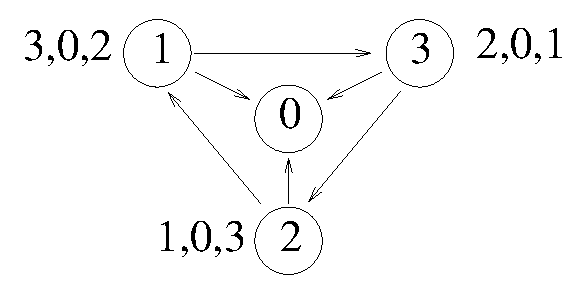
\epsfig{file=policy/figures/nexthop_osc.eps,
    width=0.4\linewidth}}\hfill 
%
\subfigure[Activation sequence]{
\parbox{0.5\linewidth}{
\vspace*{-0.75in}
{\scriptsize
\begin{tabular}{l|ccc}
Activate & 1 & 2 & 3 \\ \hline
--- & (1 0) & (2 0) & (3 2 0) \\ 
2 & (1 0) & {\bf (2 1 0)} & (3 2 0) \\
1 & {\bf (1 3 2 0)} & (2 1 0) & (3 2 0) \\
3 & (1 3 2 0) & (2 1 0) & {\bf (3 2 1 0)} \\
2 & (1 3 2 0) & {\bf (2 0)} & (3 2 1 0) \\
1 & {\bf (1 0)} & (2 0) & (3 2 1 0) \\
3 & (1 0) & (2 0) & (3 2 0)
\end{tabular}}
}}
\caption[Routing system with next-hop rankings that is not
  safe]{Next-hop rankings are not safe in this routing system.  AS 
$1$ prefers all paths through AS $3$ over the direct path to the
destination $0$ (with ties broken deterministically) and prefers the
direct path over all paths through AS $2$.  Similarly, AS $3$ prefers
all paths via AS $2$, and so forth.}
\label{fig:nexthop_osc}
\end{figure}

%% \begin{figure}
%% \begin{center}
%% \end{center}
%% \caption{Next-hop rankings are not safe.} 
%% \label{fig:nexthop_activation}
%% \end{figure}


\begin{observation}
A routing system where each node has only a next-hop ranking may
not be safe.
\end{observation}

\begin{example}
Consider Figure~\ref{fig:nexthop_osc}.  In this example,
each AS ranks every one of its neighboring ASes.
For example, AS $1$ prefers all paths that traverse AS $3$ as the
immediate next hop over all paths that traverse AS $0$ as the immediate
next hop, regardless of the number of ASes each path traverses;
similarly, AS $1$ prefers paths that traverse AS $0$ as the immediate next hop
over paths that traverse AS $2$.  Each AS readvertises its best path to
the destination to all of its neighbors (\ie, the system has no
filtering).  Now consider the activation sequence in
Figure~\ref{fig:nexthop_osc}(b); if infinitely repeated, this
activation sequence would be fair, and the routing system would
oscillate forever.  Thus, the routing system is not safe.

This system is not {\em safe}, but it is {\em stable}: for
example, the path assignment $(10, 210, 3210)$ is stable.  Nodes
2 and 3 are using paths through their most preferred nodes.  Node 1's
most preferred node, node 3, is using a path that already goes through
node 1, so node 1 is also using its most preferred consistent path.  As
every node is using its most preferred consistent path, no node will
change paths when activated, so the path assignment is stable.
\end{example}

A routing system where each node has a next-hop ranking
may not be safe, but Feigenbaum \ea showed that
there is always 
guaranteed to be at least one stable path assignment for such routing
systems \cite{Feigenbaum2004}.  However, allowing nodes to filter paths from
each other can create routing systems for which there is {\em no}
stable path assignment.


\begin{observation}
There exist routing systems with next-hop
rankings for which a stable path assignment exists, but introducing
filtering can yield a system where {\em no} stable path assignment exists.
\end{observation}


\begin{figure}
\centering
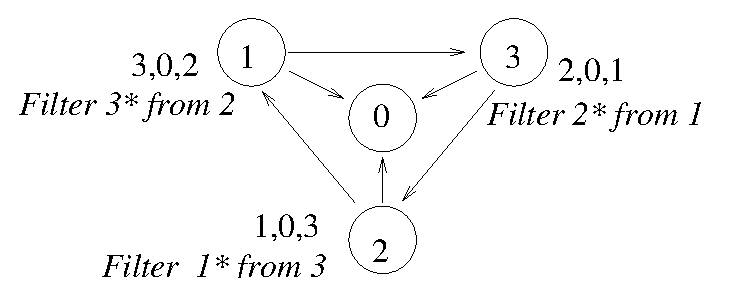
\epsfig{file=policy/figures/bg2.eps, width=0.75\columnwidth}
%}\hspace*{0.2in}
%\subfigure[Equivalent system with arbitrary rankings.]{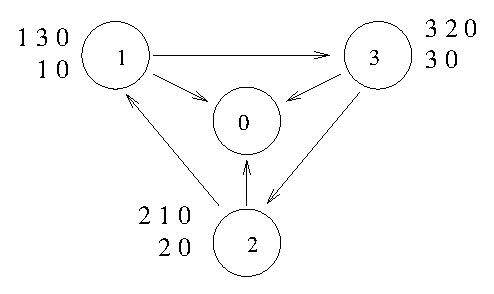
\epsfig{file=policy/figures/bg2a.eps, width=0.4\columnwidth}}
\caption[Routing system that is stable without filtering but unstable
  under filtering.]{This routing system is stable without filtering but
  unstable 
  under filtering. The figure shows a routing system with
  next-hop rankings and filtering that is equivalent to the unstable
  routing system with the rankings over paths shown in
  Figure~\ref{fig:bg1}.}
\label{fig:bg2}
\end{figure}


%% \begin{observation}[Instability of next-hop rankings under filtering]
%% For a BGP system, $(N, \prec_1^N, \ldots, \prec_N^N,
%% \F_1^N, \ldots, \F_N^N)$, if $\prec_i^N$ is a next-hop ranking
%% relation, then there exists some set of filters $\F_1^N, \ldots, \F_N^N$
%% such that the BGP system is not safe.
%% \end{observation}

\begin{example}
Consider Figure~\ref{fig:bg2}.  As before, each AS ranks every one of its neighboring ASes.  Additionally,
each AS may also declare arbitrary filtering policies.  In this
example, each AS (other than the destination) does {\em not}
readvertise any indirect path to the destination.  For example, AS $1$
does not advertise the path $1 3 0$ to AS $2$, and thus the path
$2130$ is not available to AS $2$.  Formally, we define $\F_1 =
\{130, 10\}$, $\F_2 = \{210, 20\}$, and $\F_3 = \{320, 30\}$.

The resulting routing system is
equivalent to the system in Figure~\ref{fig:bg1}, once the filtered
paths are removed from each node's ranking.  Thus, the
filtered routing 
system is unstable by the same reasoning as that from the example shown
in Figure~\ref{fig:bg1}:
for any path assignment in this routing system, at 
least one AS will have a higher ranked consistent path (and, hence,
has an incentive to deviate from the path assignment).  
%For example,
%consider the path assignment $\v{P}_1 = (130, 20, 30)$.  AS $3$
%prefers to switch paths to $320$, since $2$ is its preferred next hop
%AS.
\end{example}

Using a construction similar to that from the example in
Figure~\ref{fig:depeer}, it is 
possible to show how this example could arise in practice.  The
example demonstrates the complex interaction between filtering and
rankings---a class of rankings that guarantees stability
without filtering can be unstable under certain
filtering conditions.   
%Previous
%work has shown that placing strong restrictions on the allowable
%filtering policies can guarantee stability~\cite{Gao2001a}, but placing
%restrictions on filtering restricts an AS's ability to make autonomous
%and flexible decisions about route advertisement, as in this example.


%% Note that this example does {\em not} contradict the safety
%% conditions stipulated by Gao and Rexford~\cite{gao:01}.  If ASes $1$,
%% $2$, and $3$ are peers (the only relationship that would not induce a
%% cycle in the peer-provider relationships), then AS $0$ must either be a
%% customer, a provider, or a peer.  If $0$ is a customer, then Guideline A
%% is violated, since the other ASes strictly prefer peer routes over
%% customer routes.  If $0$ is a provider, then the Gao/Rexford export
%% constraints are violated, since ASes $1$, $2$, and $3$ each readvertiese
%% a provider route to its peers.  If $0$ is a peer, then the Gao/Rexford
%% constraints do not apply, since there is no hierarchy.

\subsection{Edge Weight-Based Rankings}
\label{ssec:ew}

\begin{figure}
\centering
\begin{psfrags}
%
\psfrag{w_10}{{\large $w_{10}$}}
\psfrag{w_20}{{\large $w_{20}$}}
\psfrag{w_30}{{\large $w_{30}$}}
\psfrag{w_12}{{\large $w_{12}$}}
\psfrag{w_23}{{\large $w_{23}$}}
\psfrag{w_31}{{\large $w_{31}$}}
%
%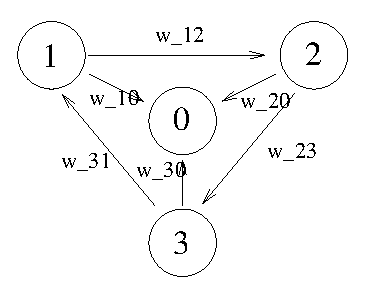
\epsfig{file=policy/figures/edgeweight.eps, width=0.35\columnwidth}
\resizebox{0.4\columnwidth}{!}{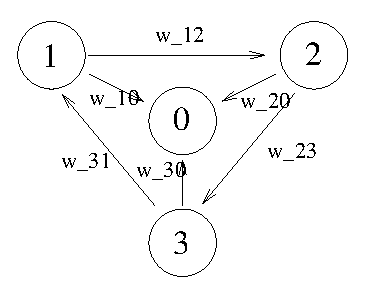
\includegraphics{policy/figures/edgeweight.eps}}
\end{psfrags}
\caption{Routing system with edge weight-based rankings.} 
\label{fig:edgeweight}
\end{figure}

There exists at least one routing system that preserves autonomy and yet
ensures safety under filtering: if each provider is allowed to choose
edge weights for its outgoing links, and each provider ranks paths based
on the sum of edge weights, the resulting ``shortest paths'' routing
system is guaranteed to be safe \cite{Griffin2002c}.  Since this result
holds for any $\F_1, \ldots, \F_N$, any routing system built in this way
is guaranteed to be safe under filtering.  In this section, we will
formulate a generalized model of such {\em edge weight-based rankings},
with both next-hop rankings and shortest path routing as special cases.
Such rankings do not allow providers to directly specify their ranking;
rather, the rankings of each provider are {\em derived} from the
strategic choices made by all providers, namely, the choices of outgoing
link weights that each provider sets.  This notion of ``derived''
rankings is a potentially useful method for ensuring autonomy in
interdomain routing protocols.

\begin{defn}[Edge weight-based rankings]
$\lb(N,\prec_1,\ldots,\prec_N, \F_1, \ldots, \F_N)$ is a routing
system with {\em edge weight-based
rankings} if there exists an assignment of edge weights $w_{ij}$ to
each ordered pair of ASes $i,j$, together with a parameter $\alpha \in
[0, 1]$, such that for each AS $i$ and paths $P_i, \hat{P}_i \in \P_i^N$
with $P_i = i i_1 \ldots i_n 0$ and $\hat{P}_i = i j_1 \ldots j_m 0$,
there holds:
\begin{multline*}
P_i \prec_i \hat{P}_i\ \ \textrm{if and only if}\ \ w_{ii_1} + \alpha
\left( \sum_{k = 1}^{n-1} w_{i_k i_{k+1}} + w_{i_n 0}\right) >
w_{ij_1} + \alpha \left(\sum_{\ell =
1}^{m-1} w_{j_\ell j_{\ell+1}} + w_{j_m 0}\right).
\end{multline*}
\end{defn}


The interpretation of this definition is as follows.  Each
node chooses edge weights for all possible outgoing links; \ie, node
$i$ chooses a weight 
$w_{ij}$ for each node $j$.  Next, node $i$ determines its rankings
by ordering all paths $P_i = i i_1 \ldots i_n 0$ in increasing order
according to their weight $w_{ii_1} + \alpha ( \sum_{k = 1}^{n-1} w_{i_k
i_{k+1}} + w_{i_n 0})$, where $\alpha$ is a global parameter used to
weight the tail of the path.  The parameter $\alpha$ allows us to
compare two extreme points: $\alpha = 1$, corresponds to shortest path
routing based on the matrix of edge weights 
$\v{w}$, while $\alpha = 0$ corresponds to next-hop rankings.
%
%
%% We now examine whether a routing system that uses only edge weight-based
%% rankings can be stable if each node acts autonomously in setting edge
%% weights for its outgoing links.  We know that routing systems where all
%% nodes have next-hop rankings can be unsafe, as well as
%% unstable under filtering; thus, when $\alpha = 0$, there exist choices
%% of edge weights by the nodes that can lead to routing systems that are
%% unsafe or unstable under filtering.  On the other hand, Griffin {\em et
%% al.} previously showed that routing systems that use shortest paths
%% routing are always safe \cite{Griffin2002c}, and their result implies
%% that such systems are in fact always safe under filtering.  Thus when
%% $\alpha = 1$, any routing system built from edge weight-based
%% rankings is guaranteed to be safe, regardless of the choices of
%% weights by the nodes.
%
A natural question to ask is whether a routing system using edge
weight-based rankings can be safe for intermediate values of
$\alpha$.  It turns out that the {\em only} edge weight-based ranking
class that can guarantee safety (and safety under filtering), regardless
of the weights chosen by each provider, is the scheme defined
by $\alpha = 1$; \ie, shortest path routing.


\begin{observation}
A routing system with edge weight-based rankings may be unstable
for any $\alpha$ where $0  < \alpha < 1$.
\end{observation}

\begin{example}
Consider the routing system shown in Figure~\ref{fig:edgeweight}.  If
the system is such that each node prefers the two-hop path to the
destination, followed by the one-hop (\ie, direct) path, followed by the
three-hop path, then the system will be unstable because its behavior
will correspond to that shown  
in Figure~\ref{fig:bg1}.  The routing system will be unstable if the
following conditions are satisfied, for all $i=1,2,3$:
%\begin{eqnarray*}
$w_{i,i+1} + \alpha w_{i+1,0}  <  w_{i,0} < w_{i,i+1} +
\alpha(w_{i+1,i+2} + w_{i+2,0})$ (for addition modulo $3$).
%w_{23} + \alpha w_{30}  <  w_{20} &<& w_{23} + \alpha(w_{31} + w_{10})\\
%w_{31} + \alpha w_{10}  <  w_{30} &<& w_{31} + \alpha(w_{12} + w_{20})
%\end{eqnarray*}
If $\alpha = 1$, these inequalities cannot be simultaneously satisfied
for any nonnegative choice of the edge weight vector $\v{w}$, which is
expected, since $\alpha =1$ corresponds to shortest path
routing.  On the other hand, if $0 < \alpha < 1$, then there are many vectors
$\v{w}$ that satisfy the inequalities above.  For example, we can choose
$w_{10} = w_{20} = w_{30} = 1$, and let $w_{12} = w_{23} = w_{31} =
x$, for any $x$ such that $(1 - \alpha)/(1+\alpha) < x < 1-\alpha$.
For this definition of $\v{w}$, all three inequalities above will be
satisfied, and thus the rankings of each node will lead to the same
oscillation shown in Figure~\ref{fig:bg1}.
\end{example}

The results in this section imply that routing protocols maybe unstable
if individual nodes may rank paths in ways that deviate even slightly
from rankings based on shortest paths routing.  Of course, the reader
should not interpret these results as saying that shortest paths routing
is the {\em only} routing protocol that will converge, since there is a
larger class of routing protocols based on strictly monotonic algebras
(of which shortest paths routing is one instance) that are
safe~\cite{Griffin2005}.  Rather, the results imply that a routing
protocol where nodes may rank paths in ways that violate the
monotonicity of shortest paths routing---even if only slightly---are may
be unstable.

